\section{Projection Operator: Continuous Fourier Expansion}
	\vspace{0.2cm}
		
	We define the projection operator denoted as $\mathcal{P}_N$ as the truncated Fourier series, i.e.,
	\begin{equation}
	\label{proyection_operator}
		\mathcal{P}_N u(x) \equiv  \displaystyle \sum_{ |n| \leq \frac {N}{2}} \hat{u}_{n} e^{inx}.
	\end{equation}	
	We will denote to $\hat{B}_N$ as the finite subset of $B = span\{e^{inx}: |n| \leq \infty \}$ on which it is projected the function, represented as follows
	\begin{align*}
		\hat{B}_{N} = span \left\{e^{inx}: |n| \leq \frac {N}{2} \right\},\hspace{0.2cm} dim(\hat{B}_{N}) = N + 1.
	\end{align*}
	Then by the orthogonality relation (\ref{ortho_phi}), it can be seen that for $u(x) \in L^2 [0, 2\pi]$
	\begin{align*}
		\langle \mathcal{P}_N u, v \rangle = \langle u, v \rangle, \hspace{3mm} \forall v \in S_N.
	\end{align*}
	This shows that $\mathcal{P}_N u$ is the orthogonal projection of $u$ upon the space of the trigonometric polynomials of degree $N$.\\
	
	Equivalently, $\mathcal{P}_N u$ is the closest element to $u$ in $\hat{B}_N$ with respect to the inner product
	\begin{align*}
		\langle u, v \rangle = \displaystyle \int_{0}^{2 \pi} u(x) \overline{v(x)} dx,
	\end{align*}
	and this also defines the norm
	\begin{align}
	\label{L2_dot}
		\| u \|^2 = \displaystyle \int_{0}^{2 \pi} |u(x)|^2 dx.
	\end{align}
	
	A full characterization of the functions for which the Fourier series is convergent is the framework of Lebesgue integration for convergence in mean. This convergence can be defined in $L^2 (0, 2 \pi)$ (square-integrable functions), also is a complex Hilbert space with inner product defined by (\ref{L2_dot}). Then for $u \in L^2 (0, 2 \pi)$ the Fourier series $F(u)$ given by (\ref{fourier_series}) is said to be convergent in mean (or $L^2$-convergent) to $u$ if
	\begin{align}
		\label{L2_mean}
		\displaystyle \int_{0}^{2 \pi} |u(x) - \mathcal{P}_N u(x) |^2 dx \rightarrow 0, \hspace{2mm} \text{as} \hspace{2mm} N \rightarrow \infty,
	\end{align}
	
	Then the Functions in $L^2 (0, 2 \pi)$ can be characterized in terms of their Fourier coefficients, according to the Riesz theorem, in the following sense. If $u \in L^2 (0, 2 \pi)$, then its Fourier series converges to $u$ in the sense of (\ref{L2_mean}), and by Parseval's identity show us that
	\begin{align}
	\label{parseval}
		\| u \|^2 = 2 \pi \displaystyle \sum^{\infty}_{-\infty} |\hat{u}_n|^2.
	\end{align}
	Conversely, if for any complex sequence $\{\hat{u}_n \}$, $n = 0, \pm 1, \dots $, and $\sum^{\infty}_{n=-\infty} |\hat{u}_n|^2 < \infty$, there exists a unique function $u \in L^2 (0, 2 \pi)$ such that its Fourier coefficients are precisely the $\hat{u}_n$$'$s for any $n$. Thus, for any function $u \in L^2 (0, 2 \pi)$ can be written as
	\begin{align}
		u = \displaystyle \sum^{\infty}_{n=-\infty} \hat{u}_n \phi_n.
	\end{align}
	
	The Riesz theorem states that the finite Fourier transform is an isomorphism between $L^2 (0, 2\pi)$ and the space $l^2$ of complex sequences $\{\hat{u}_n \}$, $n = 0, \pm1, \pm2, \dots$, such that $\sum^{\infty}_{n=-\infty} |\hat{u}_n|^2 < \infty$. The above can be summed up in the following theorem. 
	
	\begin{teor}
		 If the sum of squares of the Fourier coefficients is bounded
		\begin{align*}
			\displaystyle \sum_{ |n| \leq \infty} |\hat{u}_n|^2 < \infty
		\end{align*}
		then the truncated series converges in the $L^2$ norm
		\begin{align*}
			\|u -  \mathcal{P}_N u \|_{L^2 [0, 2\pi]} \rightarrow 0 \hspace{0.5cm} \text{as} \hspace{0.5cm} N \rightarrow \infty.
		\end{align*}
		If, moreover, the sum of the absolute values of the Fourier coefficients is bounded
		\begin{align*}
			\displaystyle \sum_{ |n| \leq \infty} |\hat{u}_n| < \infty
		\end{align*}
		then the truncated series converges uniformly 
		\begin{align*}
			\|u -  \mathcal{P}_N u \|_{L^{\infty} [0, 2\pi]} \rightarrow 0 \hspace{0.5cm} \text{as} \hspace{0.5cm} N \rightarrow \infty. 
		\end{align*}
	\end{teor}
	
	Note that if the truncated sum converges implies that the error is dominated by the tail of the series, i.e.,
	\begin{align*}
		\|u -  \mathcal{P}_N u \|^2_{L^2 [0, 2\pi]} = 2 \pi	\displaystyle \sum_{ |n| > \frac{N}{2} } |\hat{u}_n|^2,
	\end{align*}	
	and	
	\begin{align*}
		\|u -  \mathcal{P}_N u \|_{L^{\infty} [0, 2\pi]} \leq 
		\displaystyle \sum_{|n| > \frac{N}{2}} |\hat{u}_n|. 
	\end{align*}
	Thus, the error committed by replacing $u(x)$ with its $N$th-order Fourier series depends solely on how fast the expansion coefficients of $u(x)$ decay. \\
	
	To appreciate this, suppose that $u(x) \in L^2_p [0, 2 \pi]$ and that its derivative $u'(x) \in L^2_p [0, 2\pi]$, where the subscript $p$ indicate that the function is periodic. then for $n \neq 0$ we have to
	\begin{align*}
		2\pi \hat{u}_N &= \displaystyle \int_{0}^{2\pi} u(x) e^{-inx} dx \\
		&= - \frac{1}{in} (u(2\pi) - u(0)) - \frac{1}{in} \displaystyle \int_{0}^{2\pi} u'(x) e^{inx} dx, 
	\end{align*}
	therefore
	\begin{align*}
		|\hat{u}_N| \propto \frac{1}{n}.
	\end{align*}
	
	In general, if for $u(x)$ and its derivatives $(m - 1)$, and its periodic extensions are all continuous, and also if its derivative $m$th is measurable at $[0, 2 \pi]$, also known in the literature as the regularity of the function, in this particular case in $L^2_p$, we have to $\forall n \neq 0$, repeating the previous procedure successively, the behavior of Fourier coefficients $\hat{u}_n$ of $u(x)$ is similar, i.e.,
	\begin{align*}
		|\hat{u}_n| \propto \left(\frac{1}{n}\right)^m.
	\end{align*}
	
	 This is known as spectral convergence, which means that the smoother the function, the series converges faster.\\
	 
	 This result is important since it will allow us to investigate the convergence rate of the methods, which we will define in detail later. Therefore, we will focus on periodic functions expanded in Fourier series since its rapid decay of the coefficients implies that the Fourier series truncated after just a few more terms represents an exceedingly good approximation of the function. However, in practice, this decay is not exhibited until there are enough coefficients to represent all the essential structures of the function but in general, functions can be described both through their values in physical space and through their coefficients in transform space. The following examples illustrate the previous results. \\
	 
	\begin{example}
	    Consider the function $u(x) \in C^{\infty} [0, 2 \pi]$ given by
    	\begin{align}
    		\label{Example1} 
    	    u(x) = \frac{1}{5 - 4 \cos(x)}   
    	\end{align}
    	with its expansion coefficients
    	\begin{align*}
    	     \hat{u}_{n} = \frac{2^{-|n|}}{3}.
    	\end{align*}
    
    	In Figure \ref{fig1} we can clearly observe the convergence of the Fourier series and that in addition, the convergence of the approximation is almost uniform. This is due to the periodicity of the function and its derivatives.
    	
    	\begin{figure}[H]
        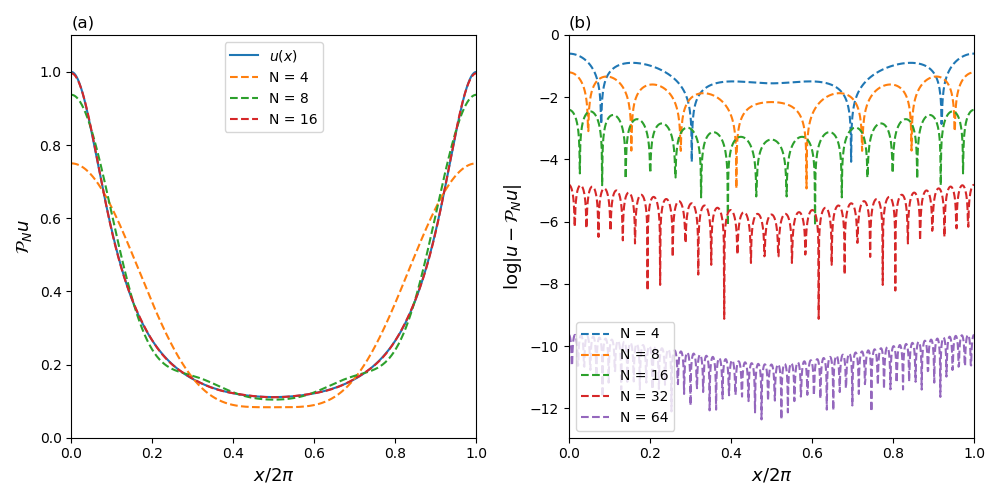
\includegraphics[width=\textwidth]{preliminaries/figures/example21.png}
        \caption{(a) Continuous Fourier series approximation of the equation (\ref{Example1}). (b) The Pointwise error of approximation.}
        \label{fig1}
        \end{figure}
	\end{example} 
	
	\begin{example}
	    The expansion coefficients of the function
    	\begin{align}
    		\label{Example2} 
    	    u(x) = \frac{\pi}{2} \sin(\frac{x}{2})
    	\end{align}
    	are given by
    	\begin{align*}
    	     \hat{u}_{n} = \frac{1}{(1 - 4n^2)}.
    	\end{align*}
    	
    	Note that is infinitely differentiable in $[0, 2 \pi]$, but $u'(0) \ne u' (2 \pi)$. In Figure \ref{fig2} we can see that the convergence is much slower than in the Example \ref{Example1}, as expected	
    	\begin{figure}[H]	
        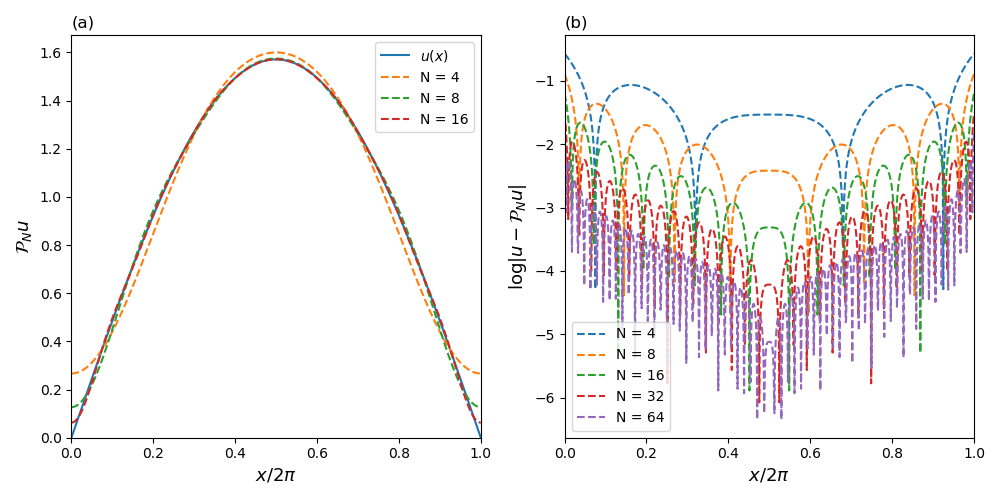
\includegraphics[width=\textwidth]{preliminaries/figures/example22.png}
        \caption{(a) Continuous Fourier series approximation of the equation (\ref{Example2}). (b) The Pointwise error of approximation for increasing resolution.}
        \label{fig2}
    	\end{figure}
	\end{example} 
	
	\subsection{Differentiation of the Continuous Expansion}

	To find solutions of partial differential equations using the spectral methods, in addition to approximating a function $u(x)$ by the finite Fourier series $\mathcal{P}_N u$, we also need to obtain its derivatives. Due to the linearity of the derivative and that these functions are exponential, we can easily obtain the derivatives of $\mathcal{P}_N u$ by simply differentiating the basis functions term by term. Therefore, if we have the following series truncated \\
 	\begin{align*}
   		\mathcal{P}_N u(x) =  \displaystyle \sum_{ |n| \leq \frac {N}{2}} \hat{u}_{n} e^{inx},
   	\end{align*}
    from this, we can get
   	\begin{align*}
   		\frac{d^q}{dx^q} \mathcal{P}_N u(x) = \displaystyle \sum_{ |n| \leq \frac {N}{2}} \hat{u}_{n} \frac{d^q}{dx^q} e^{inx} = \displaystyle \sum_{ |n| \leq \frac {N}{2}} (in)^q \hat{u}_{n}e^{inx}.
   	\end{align*}
    Therefore the projection and differentiation operators commute, i.e.,
    	\begin{align*}
    	\mathcal{P}_N \frac{d^q}{dx^q} u = \frac{d^q}{dx^q}\mathcal{P}_N u.
    	\end{align*}
    This property implies that for any differentiation operator $\mathcal{L}$ with constant coefficients,	
    	\begin{align*}
    	\mathcal{P}_N \mathcal{L} (I - \mathcal{P}_N)u
    	\end{align*}
     vanishes, which known as the truncation error. Thus, the Fourier approximation to the equation $u_t = \mathcal{L}u$ is exactly the projection of the analytic solution. 

    \subsection{Approximation theory for Continuous Expansion.}
    
    The behavior of the functions and their derivatives that we have shown is relevant when the solutions of the differential equations are approximated using spectral methods since it allows us to investigate how fast and precise they can be. In this subsection, we will present these properties based in \cite{gottlieb2007} as detailed as possible some useful results for our main objective regarding the analysis of the projection operator already defined above. \\
    
    When using the Fourier approximation to discretize the spatial part of the equation
    \begin{align*}
        u_t = \mathcal{L}u,
    \end{align*}
    it is important that our approximation, both to $u$ and to $\mathcal{L}u$, be accurate,i.e., we must consider not only the difference between $u$ and $\mathcal{P}_N u$ if not also the distance between $\mathcal{L} u$ and $\mathcal{L} \mathcal{P}_N u$, measured in an appropriate norm. This is because the actual rate of convergence is determined by the truncation error    
    \begin{align*}
    	\mathcal{P}_N \mathcal{L} (I - \mathcal{P}_N)u.
    \end{align*}
   	Thus, the error is determined not only by the behavior of the Fourier approximations of the function but also of its derivatives, as we have seen previously. Therefore, the Sobolev $q$-norm denoted by $H^q_p [0, 2\pi]$, It is appropriate to estimate the truncation error since it measures the smoothness of the derivatives and the function. This norm is defined as follows
    \begin{align}
    \label{sobolev_norm}
    	 \|u\|^2_{H^q_p [0, 2\pi]} = \displaystyle \sum^{q}_{m=0} \int^{2\pi}_{0} \left| u^m (x) \right|^2 dx.
    \end{align}
    The subscript $p$ indicates the fact that all functions are periodic. By substituting the Fourier expansion for each derivative in (\ref{sobolev_norm}), the Sobolev norm can be written as
    	\begin{align*}
    	    \|u\|^2_{H^q_p [0, 2\pi]} = 2\pi \displaystyle \sum^{q}_{m=0} \sum_{|n| \leq \infty} |n|^{2m} |\hat{u}_n|^2 = 2\pi \sum_{|n| \leq \infty} \left(\sum^{q}_{m=0} |n|^{2m} \right) |\hat{u}_n|^2,
    	\end{align*}
    where the interchange of the summation is allowed provided $u(x)$ has sufficient smoothness. \\
    
   Before starting the analysis, without loss of generality, we first consider the continuous Fourier series given by
        \begin{align*}
            \displaystyle \mathcal{P}_{2N} u(x) = \sum_{|n| \leq N} \hat{u}_n e^{in x}.
        \end{align*}
    The first important result is the estimate in $L^2$ for the distance between $u$ and its trigonometric approximation $\mathcal{P}_{2N} u$, which shows everything we've seen previously. 
    \\
    \begin{teor}
    \label{estimating_error_PN_L2}	
    For any $u(x) \in H_p^r [0, 2\pi]$, there exists a positive constant $C$, independent of $N$, such that
        \begin{align*}
    	    \|u - \mathcal{P}_{2N} u \|_{L^2 [0, 2\pi]} \leq C N^{-q} \|u^{(q)}\|_{L^2 [0, 2\pi]},
    	\end{align*}
    provided $0 \leq q \leq r$.
    \end{teor}
    \begin{proof}	
    By Parseval’s identity given by (\ref{parseval}) we get
    	\begin{align*}
    	    \|u - \mathcal{P}_{2N} u \|^2_{L^2 [0, 2\pi]} = 2\pi \displaystyle \sum_{|n| > N} |\hat{u}_n|^2.
    	\end{align*}
    We rewrite this summation as follows
    	\begin{align*}
    	    \displaystyle \sum_{|n| > N} |\hat{u}_n|^2 &= \sum_{|n| > N} \frac{n^{2q}}{n^{2q}} |\hat{u}_n|^2 \\
    	    &\leq N^{-2q} \sum_{|n| > N} n^{2q} |\hat{u}_n|^2 \\
    	    &\leq N^{-2q} \sum_{|n| \geq 0} n^{2q} |\hat{u}_n|^2 \\
    	    &= \frac{1}{2\pi} N^{-2q} \|u^{(q)}\|^2_{L^2 [0, 2\pi]}.
    	\end{align*}
    Putting all the above together and taking out the square root, we get our result.
	\end{proof}
    
    \noindent Note that the smoother the function, the larger the value of $q$ and therefore, the better the approximation, as seen before. Now let's notice the following. Suppose that $u(x)$ is analytical, so we have to
    	\begin{align*}
    		 u^{(q)} = \displaystyle 
    		 \sum_{ |n| \leq \infty} (in)^q \hat{u}_{n}e^{inx}.
    	\end{align*}
    Since $u^{(q)} \in W^q_p$, and by (\ref{parseval})
        \begin{align*}
            \|u^{(q)}\|_{L^2 [0, 2\pi]} = \sum_{ |n| \leq \infty} |n|^{2q} |\hat{u}_{n}|^2 \leq C q! \sum_{ |n| \leq \infty} |\hat{u}_{n}|^2 \leq C q! \| u \|_{L^2 [0, 2\pi]},
        \end{align*}
    and so by the previous theorem
        \begin{align*}
            \|u - \mathcal{P}_{2N} u \|_{L^2 [0, 2\pi]} \leq  N^{-q} \|u^{(q)}\|_{L^2 [0, 2\pi]} \leq C \frac{q!}{N^{q}} \| u \|_{L^2 [0, 2\pi]}.
        \end{align*}
    Using Stirling’s formula, $q! \sim q^q e^{-q}$, and assuming that $q \propto N$, we obtain
        \begin{align*}
            \|u - \mathcal{P}_{2N} u \|_{L^2 [0, 2\pi]} \leq \sim C \left(\frac{q}{N}\right)^q e^{-q} \| u \|_{L^2 [0, 2\pi]} \sim K e^{-c N} \| u \|_{L^2 [0, 2\pi]}.
        \end{align*}
    Thus, for an analytic function, its spectral convergence is exponential convergence. \\
    
    We must not forget that the theory we have previously presented is with the assumption that the functions and their derivatives are all periodic. But it is possible to do a similar analysis considering some other class of functions, such as functions that vanish at the borders. However, these kinds of functions belong to spaces very similar to those we have studied, and it is possible to use the same results.